% HPC Workload Characterisation Survey — introductory slides
% Build:  cd slides && latexmk -xelatex survey_intro.tex
\documentclass[aspectratio=169,11pt]{beamer}
\usetheme[progressbar=frametitle,numbering=fraction,block=fill]{metropolis}
\usepackage{booktabs}
\usepackage{tabularx}
\usepackage{graphicx}
\usepackage{tikz}
\usetikzlibrary{arrows.meta,positioning,shapes.geometric,calc}
\usepackage{fontawesome5}

\definecolor{iiser}{HTML}{1A3A5C}
\definecolor{soft}{HTML}{EEF3F8}
\definecolor{accent}{HTML}{2E6DA4}
\definecolor{note}{HTML}{B35C00}
\setbeamercolor{frametitle}{bg=iiser}
\setbeamercolor{progress bar}{fg=accent}
\setbeamercolor{block title}{bg=soft,fg=iiser}
\setbeamercolor{block body}{bg=soft!50}

% Placeholder to be filled in before presenting
\newcommand{\TBD}[1]{\textcolor{note}{\textbf{[#1]}}}
\newcommand{\term}[1]{\textbf{\textcolor{iiser}{#1}}}
\renewcommand{\arraystretch}{1.25}
% A job drawn as a bar from x=#1 to x=#2 at height #3 (pattern diagram)
\newcommand{\jobbar}[3]{\draw[job] (#1,#3-0.2) rectangle (#2,#3+0.2);}

\title{HPC Workload Characterisation Survey}
\subtitle{Purpose, process and a guide to the form}
\author{HPC Users' Committee}
\institute{IISER Bhopal}
\date{\today}

\begin{document}

\maketitle

% ---------------------------------------------------------------------------
\section{Purpose and scope}

\begin{frame}{Why this survey}
  \begin{itemize}\setlength{\itemsep}{2pt}
    \item Understand the \term{computing workloads} of research groups across the institute.
    \item See how well \term{Gargi} and \term{Raman} serve present needs, and where they do not.
    \item Identify problems --- resource limits, usage policies, software, storage --- that \term{can be resolved}.
    \item Plan for \term{growth} over the next few years.
  \end{itemize}
  \medskip
  \begin{block}{The principle}
    You describe what you observe. The committee applies agreed, transparent tests.\\
    You are not asked to justify your research or to judge your own priority.
  \end{block}
\end{frame}

\begin{frame}{Scope}
  \begin{columns}[T]
    \column{0.48\textwidth}
    \textbf{The survey covers}
    \begin{itemize}
      \item what you run, and how
      \item the resources your jobs use
      \item problems you have met, on any system
      \item which of those arose on Gargi or Raman
      \item expected growth
    \end{itemize}
    \column{0.48\textwidth}
    \textbf{It does not}
    \begin{itemize}
      \item rank groups or research areas
      \item assign queues or priorities
      \item decide who may use the clusters
      \item treat ``Don't know'' as ``No''
    \end{itemize}
  \end{columns}
  \vfill
  \small Experience on national facilities, collaborators' clusters or the cloud counts equally.
  Little or no use of the present clusters is \emph{not} evidence of little need.
\end{frame}

\begin{frame}{Issues the survey is designed to capture}
  Some situations users have described, in general terms:
  \medskip
  \begin{itemize}
    \item A long run stops at the wall-time limit and restarts from an earlier point.
    \item Short test jobs wait in the queue as long as large production runs.
    \item A calculation needs more nodes than any queue allows, so it runs elsewhere.
    \item A code that runs faster on more nodes is held to fewer by queue limits.
    \item A required library or version is not available on the cluster.
    \item Intermediate files outgrow the scratch space available to a job.
    \item Work moves off a cluster after a change in its usage rules.
  \end{itemize}
  \vfill
  \small The form records such issues as facts, \textbf{separately for Gargi and for Raman},
  so that each can be traced to a resource, a policy or a missing piece of software.
\end{frame}

% ---------------------------------------------------------------------------
\section{Who fills it in}

\begin{frame}{Who fills in the form, and who can help}
  \begin{columns}[T]
    \column{0.5\textwidth}
    \textbf{One submission per research group}
    \begin{itemize}
      \item the PI, or
      \item a group member who runs the calculations --- often the person who knows the details best
    \end{itemize}
    The PI receives a copy of the confirmation.
    \column{0.46\textwidth}
    \textbf{Help is available}
    \begin{itemize}
      \item A volunteer in each department can help with the technical questions.
      \item Department contacts will be informed separately
    \end{itemize}
  \end{columns}
  \vfill
  \begin{block}{``Don't know'' is always a valid answer}
    Estimates are welcome when marked as estimates. Incomplete technical knowledge does not disadvantage a submission.
  \end{block}
\end{frame}

\begin{frame}{Before you start}
  \begin{columns}[T]
    \column{0.55\textwidth}
    \textbf{Useful to have at hand}
    \begin{itemize}
      \item the main codes or applications you run
      \item for the heaviest job of each: nodes, cores or GPUs, memory, wall time
      \item roughly how many such jobs per year
      \item storage you use, and any problems you have met
    \end{itemize}
    \column{0.40\textwidth}
    \textbf{Practicalities}
    \begin{itemize}
      \item \faClock[regular]\; about \textbf{20--30 minutes}
      \item fill the sections \textbf{in order}: answers decide later questions
      \item the draft is saved in your browser as you go
    \end{itemize}
  \end{columns}
\end{frame}

% ---------------------------------------------------------------------------
\section{Terms used in the form}

\begin{frame}{Terms (1/2)}
  \small
  \begin{tabularx}{\textwidth}{@{}l X@{}}
    \toprule
    \term{Job} & One submission to the scheduler (one \texttt{sbatch}). \\
    \term{Node} & One server in the cluster; it has many cores, and may have GPUs. \\
    \term{Core} & One processing unit. A job's cores = nodes $\times$ cores used per node. \\
    \term{Wall time} & How long a job runs, from start to finish --- \emph{excluding} time waiting in the queue. \\
    \term{Queue wait} & Time from submission until the job starts running. \\
    \term{Calendar time} & From submitting the first job to the last one finishing, waits included. \\
    \bottomrule
  \end{tabularx}
  \vfill
  \normalsize
  Example: a job submitted at 9:00 starts at 13:00 and ends at 21:00.\\
  Queue wait = 4\,h \quad Wall time = 8\,h \quad Calendar time = 12\,h
\end{frame}

\begin{frame}{Terms (2/2)}
  \footnotesize\renewcommand{\arraystretch}{1.15}
  \begin{tabularx}{\textwidth}{@{}l X@{}}
    \toprule
    \term{Core-hours} & Cores $\times$ wall time. 2 nodes $\times$ 128 cores for 10\,h = 2{,}560 core-hours. \\
    \term{GPU-hours} & GPUs $\times$ wall time. 4 GPUs for 6\,h = 24 GPU-hours. \\
    \term{Wall-time limit} & The longest a job may run in a queue. Present limits: 72\,h (multi-node CPU), 168\,h (single node), 24\,h (GPU). \\
    \term{Checkpoint/restart} & A job saves its state and can continue later without repeating completed work. \\
    \term{Home / scratch} & Home keeps files between jobs; scratch is fast working space for files a job reads and writes while it runs. \\
    \term{Doubling test} & Run the same calculation on $N$ and $2N$ cores and compare wall times (e.g.\ 10\,h $\to$ 6\,h is 0.6$\times$). \\
    \bottomrule
  \end{tabularx}
\end{frame}

\begin{frame}{How jobs are organised}
  \small
  \begin{tabularx}{\textwidth}{@{}l X X@{}}
    \toprule
    \textbf{Pattern} & \textbf{Meaning} & \textbf{For example} \\
    \midrule
    \term{Stand-alone} & single calculations, each complete in one job & one simulation or analysis per job \\
    \term{Independent jobs} & many jobs that do not depend on each other & parameter sweeps, ensembles, screening \\
    \term{Sequential chain} & each job needs the previous job's output & preparation $\to$ main run $\to$ analysis, as separate jobs \\
    \term{Split calculation} & one calculation longer than the limit, continued over several jobs & a long run restarted from its checkpoint \\
    \term{Campaign} & many heavy jobs running together toward one result & coupled runs that must progress at the same time \\
    \bottomrule
  \end{tabularx}
  \vfill
  \normalsize Several can apply. Steps run inside \emph{one} job script are one stand-alone job.
\end{frame}

\begin{frame}{The patterns at a glance}
  \centering
  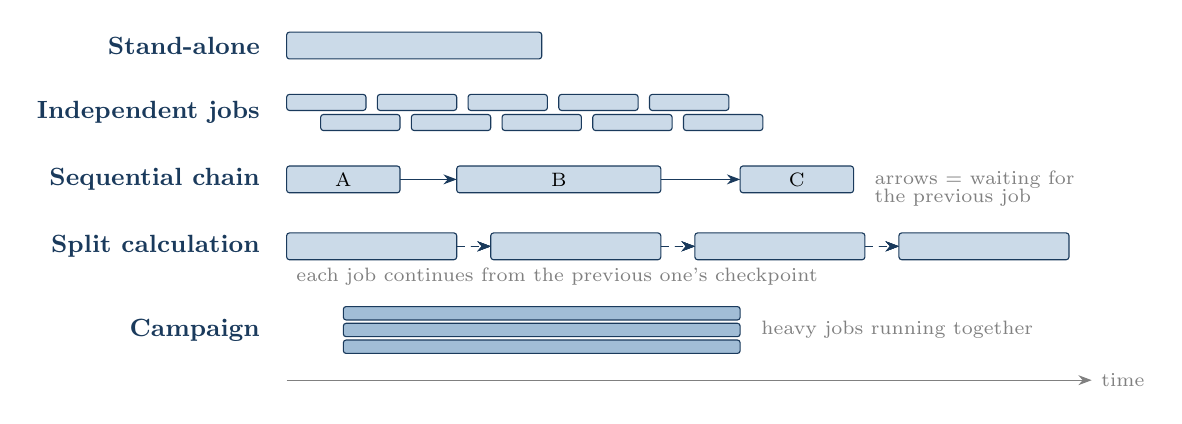
\begin{tikzpicture}[x=0.72cm,y=0.85cm]
    \tikzset{job/.style={draw=iiser,fill=accent!25,rounded corners=1pt},
             lab/.style={anchor=east,font=\small\bfseries,text=iiser},
             note/.style={anchor=west,font=\scriptsize,text=gray}}
    % stand-alone
    \node[lab] at (-0.3,5) {Stand-alone};          \jobbar{0}{4.5}{5}
    % independent jobs
    \node[lab] at (-0.3,4) {Independent jobs};
    \foreach \x in {0,1.6,3.2,4.8,6.4} {\draw[job] (\x,4.03) rectangle (\x+1.4,4.27); \draw[job] (\x+0.6,3.73) rectangle (\x+2.0,3.97);}
    % chain
    \node[lab] at (-0.3,3) {Sequential chain};
    \jobbar{0}{2.0}{3} \jobbar{3.0}{6.6}{3} \jobbar{8.0}{10.0}{3}
    \node[font=\scriptsize] at (1.0,3) {A}; \node[font=\scriptsize] at (4.8,3) {B}; \node[font=\scriptsize] at (9.0,3) {C};
    \draw[-{Stealth},iiser] (2.0,3) -- (3.0,3); \draw[-{Stealth},iiser] (6.6,3) -- (8.0,3);
    % split calculation
    \node[lab] at (-0.3,2) {Split calculation};
    \foreach \x in {0,3.6,7.2,10.8} \jobbar{\x}{\x+3.0}{2}
    \foreach \x in {3.0,6.6,10.2} \draw[-{Stealth},iiser,densely dashed] (\x,2) -- (\x+0.6,2);
    \node[note] at (0,1.55) {each job continues from the previous one's checkpoint};
    % campaign
    \node[lab] at (-0.3,0.75) {Campaign};
    \foreach \y in {1.0,0.75,0.5} \draw[job,fill=accent!45] (1.0,\y-0.1) rectangle (8.0,\y+0.1);
    \node[note] at (8.2,0.75) {heavy jobs running together};
    % axis
    \draw[-{Stealth},gray] (0,0) -- (14.2,0) node[right,font=\scriptsize,text=gray]{time};
    \node[note] at (10.2,3) {arrows = waiting for};
    \node[note] at (10.2,2.72) {the previous job};
  \end{tikzpicture}
\end{frame}

% ---------------------------------------------------------------------------
\section{The form}

\begin{frame}{Layout of the form}
  \small\renewcommand{\arraystretch}{1.12}
  \begin{tabularx}{\textwidth}{@{}c l X@{}}
    \toprule
    & \textbf{Section} & \textbf{Purpose} \\
    \midrule
    A & About your group & contact details; who is filling in the form \\
    B & Your HPC experience & systems used; problems met --- anywhere, then on Gargi and on Raman \\
    C & Your workloads & one entry per code and kind of job: size, wall time, jobs per year, pattern \\
    D & Details for each code & short follow-up panels, only where an entry calls for them \\
    E & Storage, testing, interactive use & home space; short test and interactive sessions \\
    F & Queue and turnaround & only if queue waits or capacity problems were reported \\
    G & Growth and closing & expected growth; optional help with benchmarks; comments \\
    \bottomrule
  \end{tabularx}
  \vfill
  \normalsize Required answers are marked \textcolor{red}{*}; each has ``Don't know'' where it applies.
\end{frame}

\begin{frame}{Section B --- problems on each cluster}
  \begin{columns}[c]
    \column{0.60\textwidth}
    \centering
\includegraphics[width=\linewidth]{figures/b_gargi.png}
    \column{0.36\textwidth}
    \begin{itemize}
      \item First: problems met on \emph{any} system.
      \item Then: which of them arose on \textbf{Gargi} --- and, in a separate question, on \textbf{Raman}.
      \item Their hardware and usage policies differ.
    \end{itemize}
  \end{columns}
\end{frame}

\begin{frame}{Section B --- did the problems keep work away?}
  \begin{columns}[c]
    \column{0.60\textwidth}
    \centering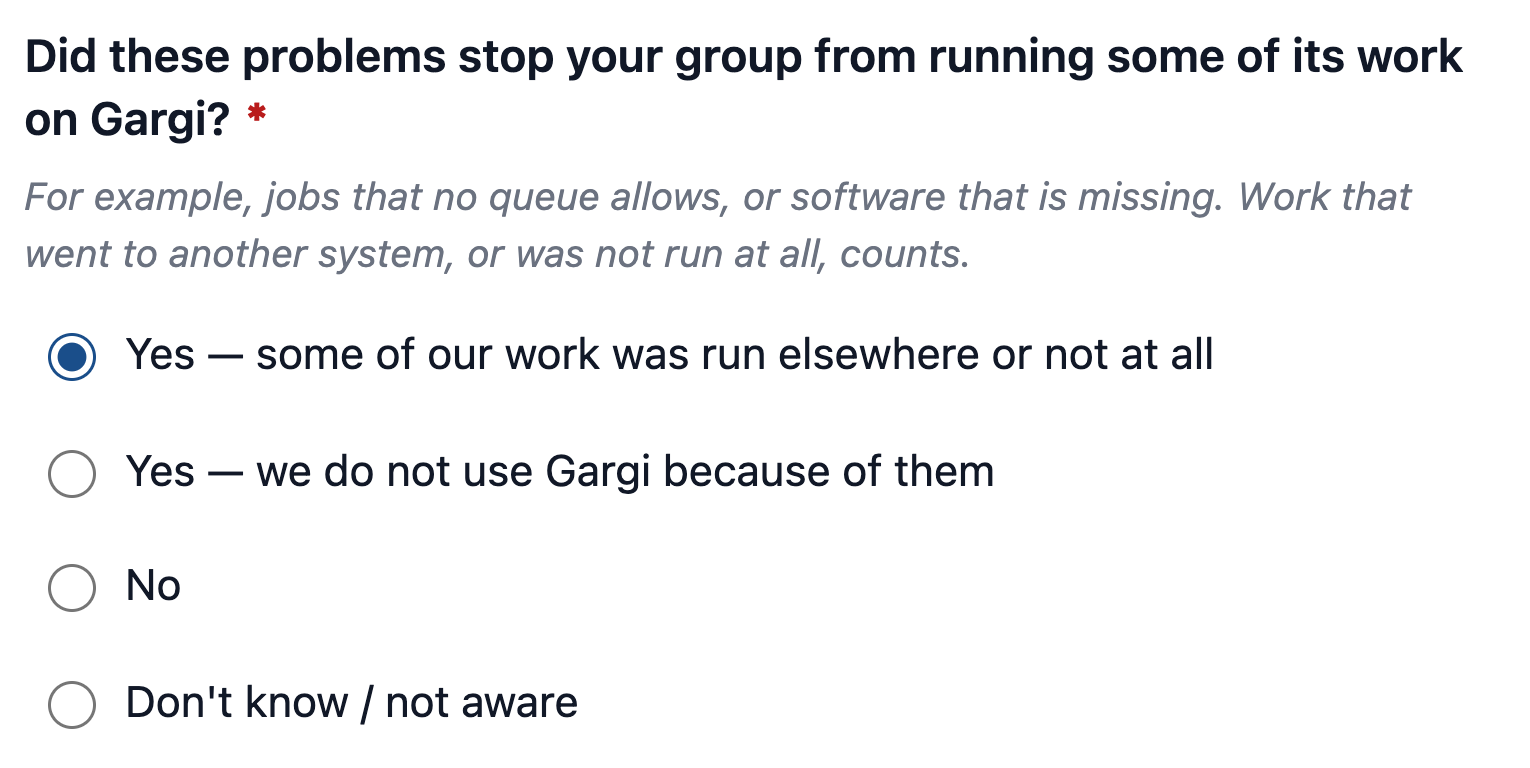
\includegraphics[width=\linewidth]{figures/b_nonuse.png}
    \column{0.36\textwidth}
    \begin{itemize}
      \item Asked after each cluster's problems.
      \item Work run elsewhere, or not run at all, is recorded --- it is demand the clusters did not see.
    \end{itemize}
  \end{columns}
\end{frame}

\begin{frame}{Section C --- one entry per code and kind of job}
  \begin{columns}[c]
    \column{0.60\textwidth}
    \centering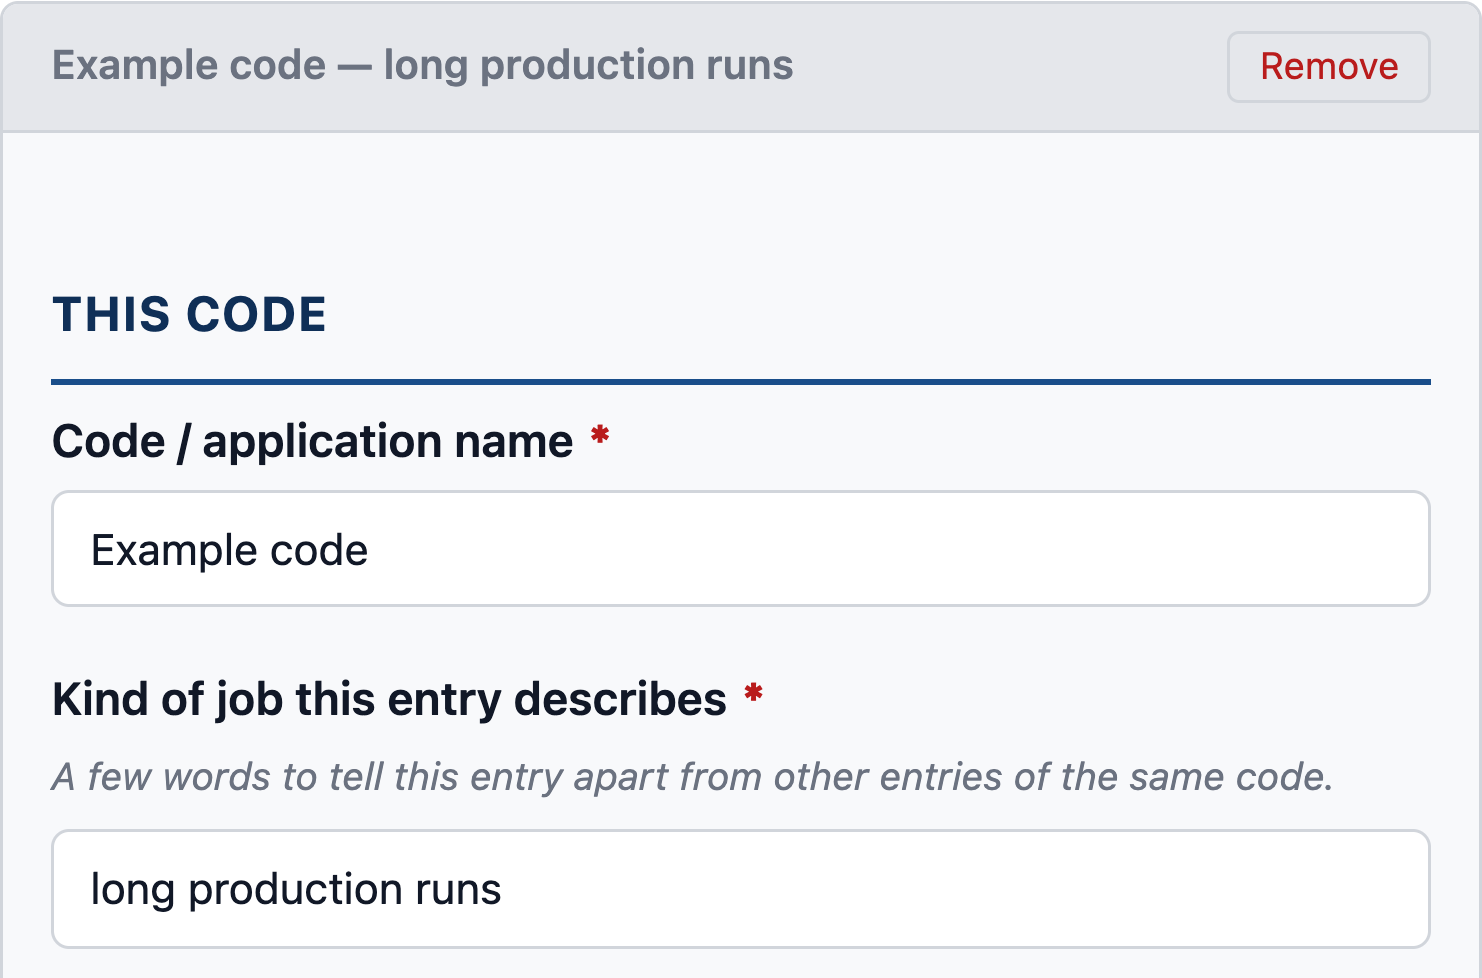
\includegraphics[width=\linewidth]{figures/c_entry.png}
    \column{0.36\textwidth}
    \begin{itemize}
      \item The same code can have several entries for quite different kinds of jobs.
      \item Describe the \textbf{heaviest} job of each entry; the committee works out the totals.
      \item Jobs run elsewhere count too.
    \end{itemize}
  \end{columns}
\end{frame}

\begin{frame}{Section C --- how the jobs are organised}
  \centering
  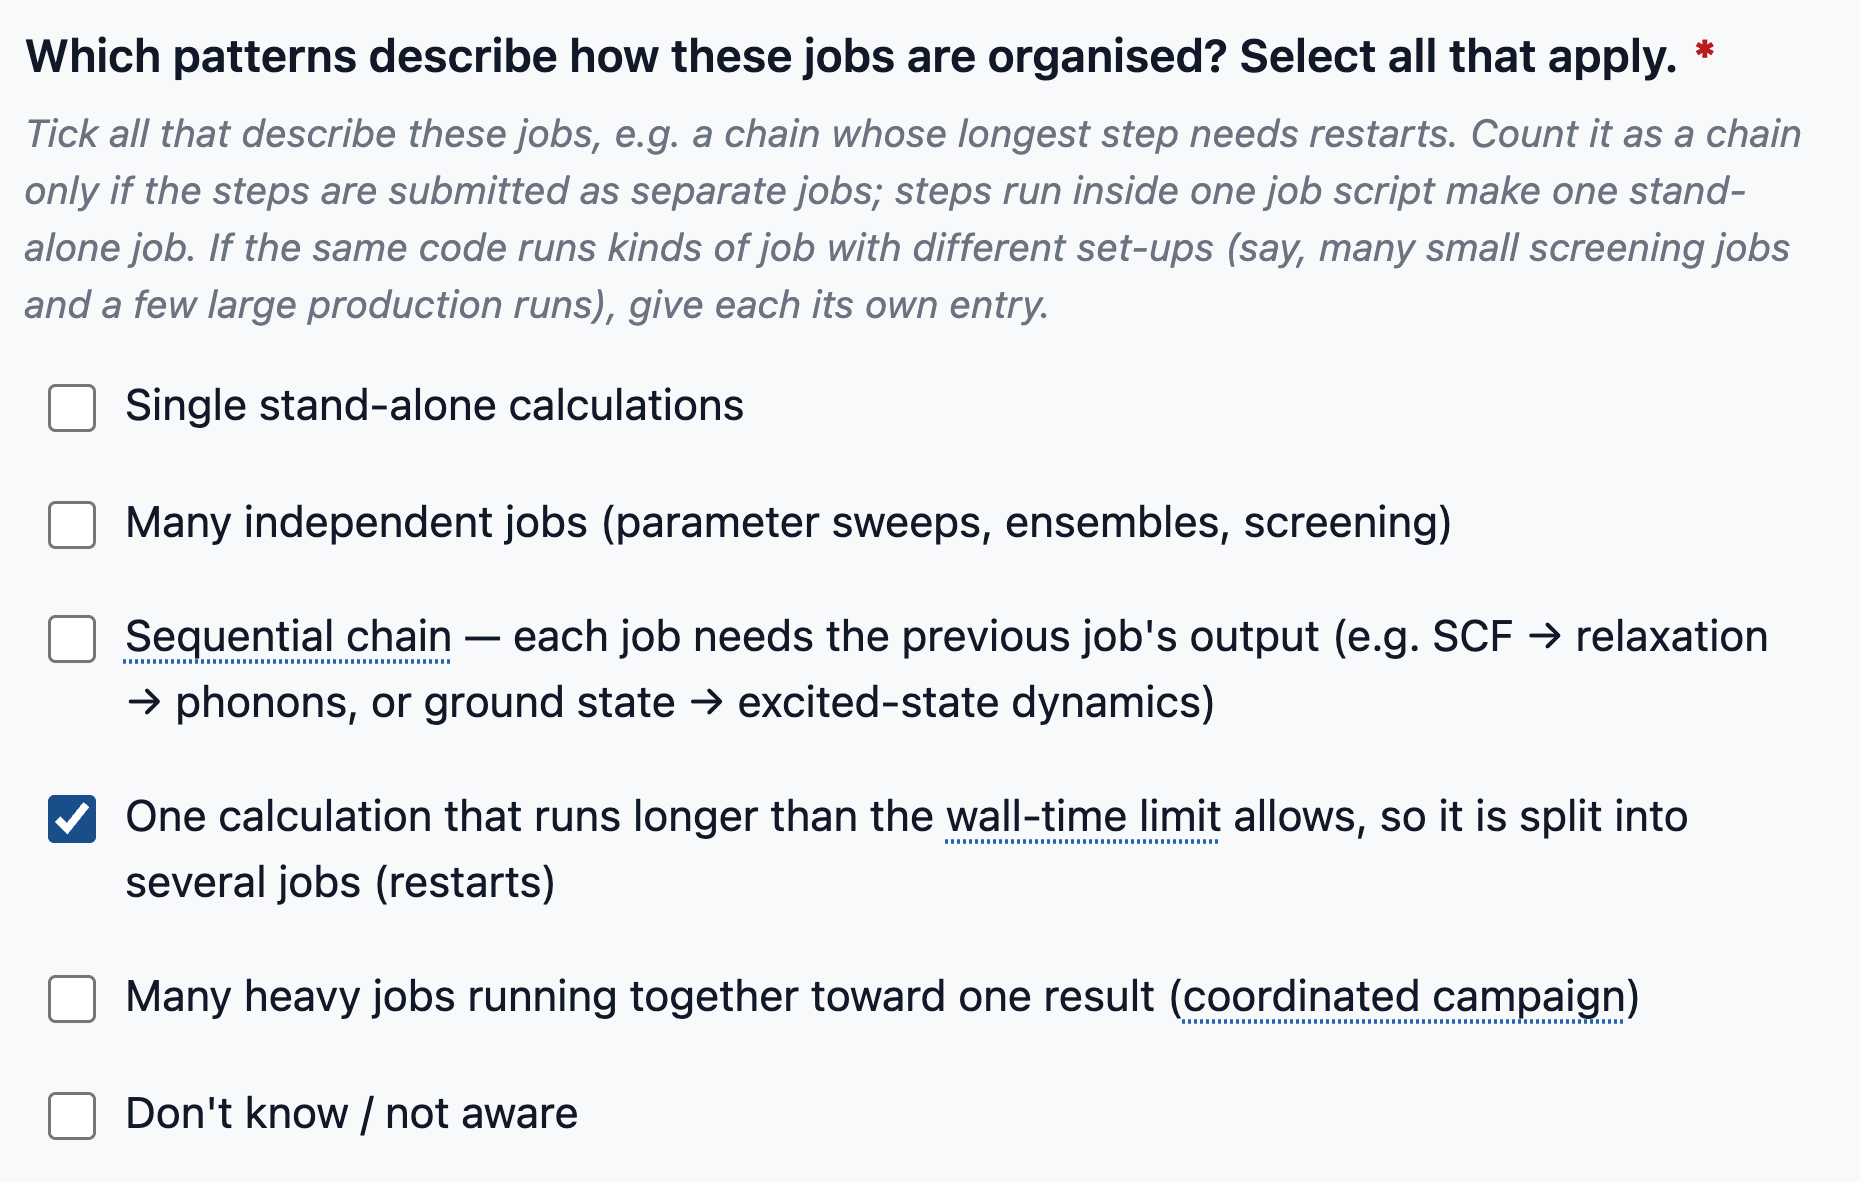
\includegraphics[height=6.4cm]{figures/c_patterns.png}
\end{frame}

\begin{frame}{Section D --- follow-up panels}
  \footnotesize\renewcommand{\arraystretch}{1.12}
  \begin{tabularx}{\textwidth}{@{}l X X@{}}
    \toprule
    \textbf{Panel} & \textbf{Opens when an entry \ldots} & \textbf{Asks about} \\
    \midrule
    Job organisation & uses independent jobs, a chain, a split calculation or a campaign & batch size; length of a sequence; campaign size \\
    Long runs & exceeds a wall-time limit, or is linked to jobs stopped by it & checkpoint/restart; jobs stopped \\
    More cores & is long or large, or is linked to node-count limits & effect of doubling cores; measured runs \\
    Memory & needs more than a standard node, or ran out of memory & standard nodes; spreading memory \\
    GPU & runs on GPUs, or is linked to GPU access & GPU model, memory, interconnect \\
    Files and scratch & reads or writes large volumes, or is linked to scratch & I/O pattern; how long files stay \\
    \bottomrule
  \end{tabularx}
  \vfill
  \normalsize Each panel appears once per entry, whatever opened it, and says why.
\end{frame}

\begin{frame}{Section D --- a panel}
  \begin{columns}[c]
    \column{0.68\textwidth}
    \centering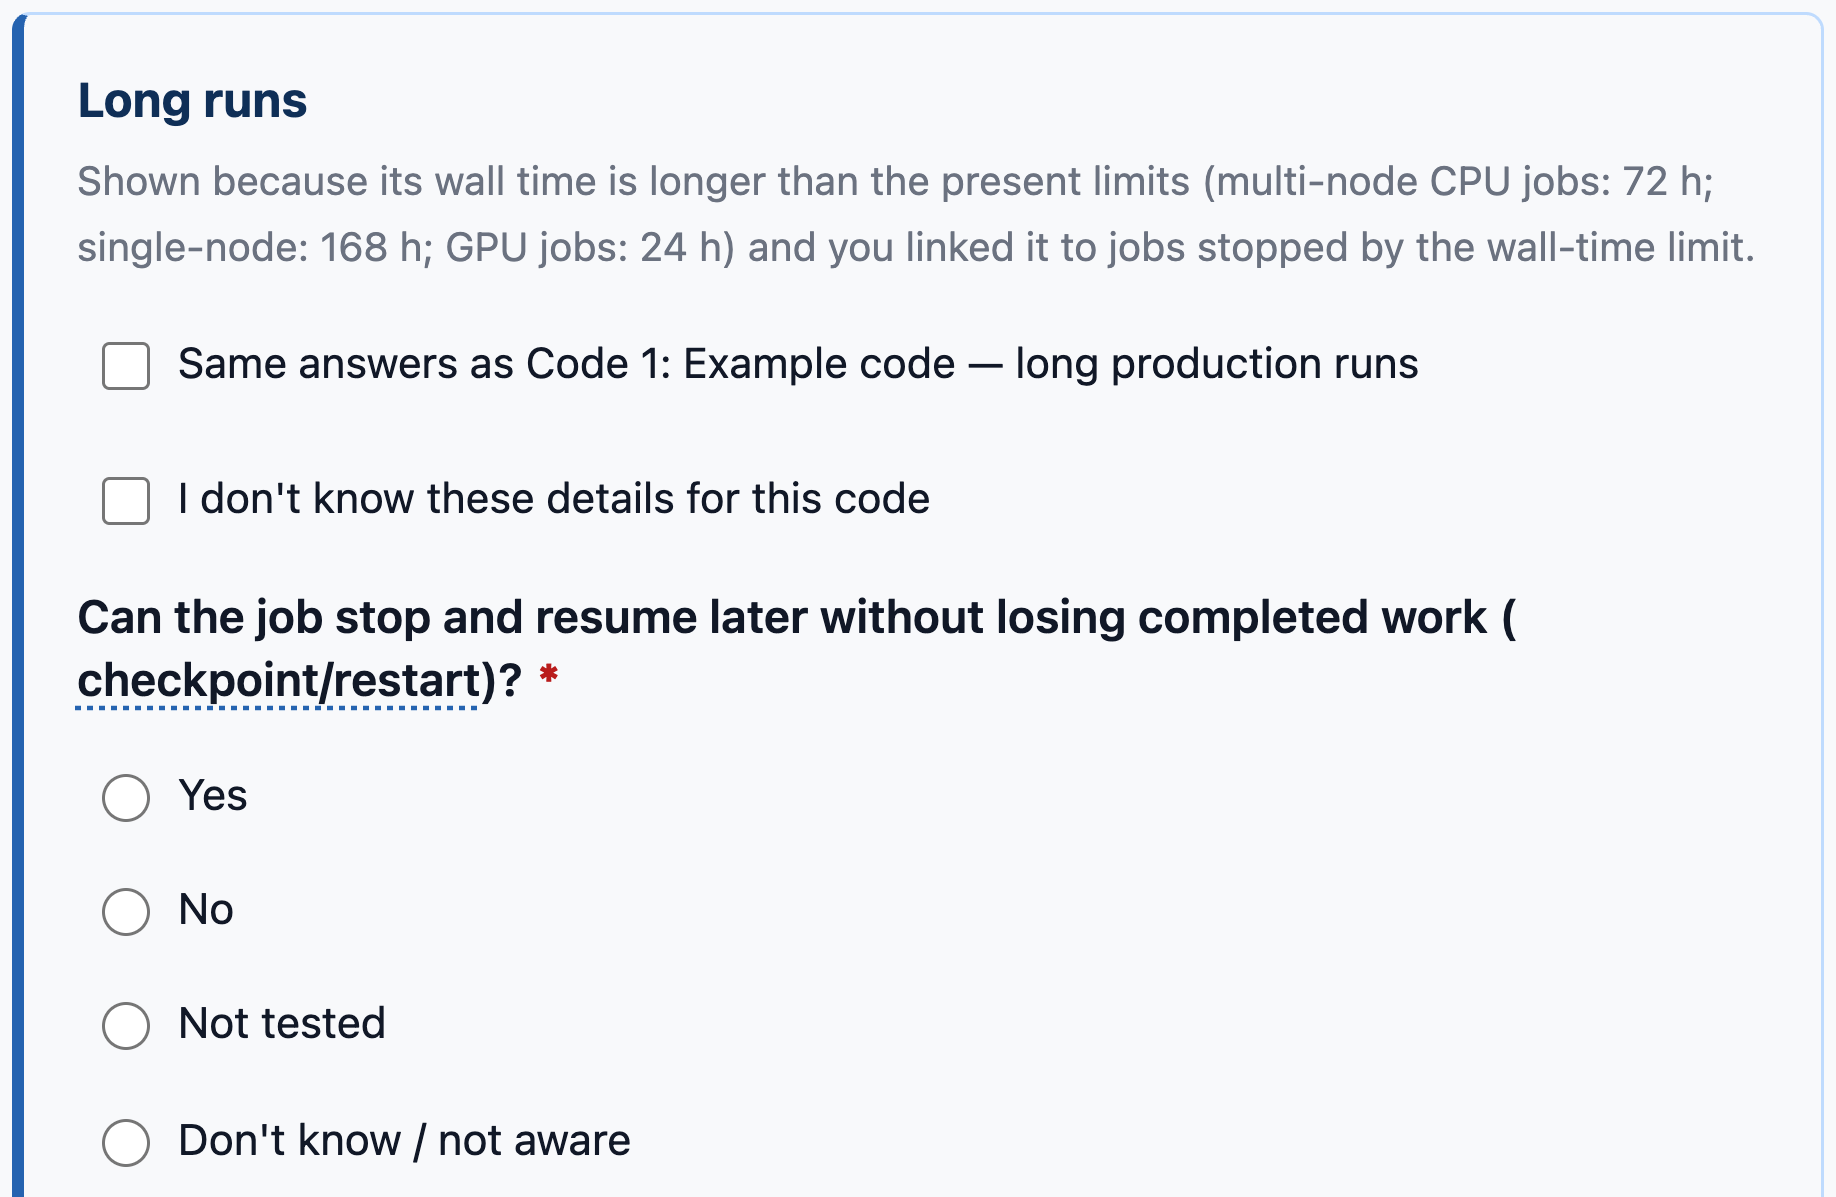
\includegraphics[height=6.3cm]{figures/d_panel.png}
    \column{0.30\textwidth}
    \small
    \begin{itemize}
      \item ``Shown because \ldots'' gives every reason.
      \item \emph{Same answers as \ldots} reuses an earlier entry of the same code.
      \item \emph{I don't know these details} is a valid answer.
    \end{itemize}
  \end{columns}
\end{frame}

% ---------------------------------------------------------------------------
\section{Submission and evaluation}

\begin{frame}{Submitting}
  \centering
  \resizebox{0.97\textwidth}{!}{%
  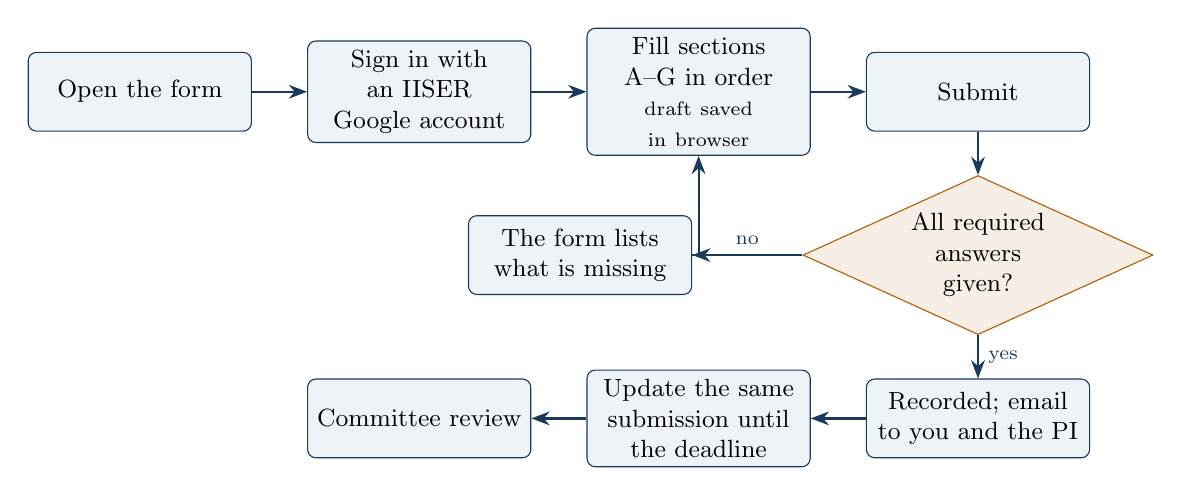
\begin{tikzpicture}[node distance=0.5cm and 0.7cm,
      stp/.style={draw=iiser,fill=soft,rounded corners=3pt,align=center,font=\small,minimum height=1.0cm,text width=2.6cm},
      check/.style={draw=note,fill=note!10,diamond,aspect=2.2,align=center,font=\small,inner sep=1pt,text width=1.9cm},
      arr/.style={-{Stealth},thick,iiser}]
    \node[stp] (open) {Open the form};
    \node[stp,right=of open] (sign) {Sign in with an IISER Google account};
    \node[stp,right=of sign] (fill) {Fill sections A--G in order\\{\scriptsize draft saved in browser}};
    \node[stp,right=of fill] (submit) {Submit};
    \node[check,below=0.55cm of submit] (ok) {All required answers given?};
    \node[stp,left=1.4cm of ok] (fix) {The form lists what is missing};
    \node[stp,below=0.55cm of ok] (rec) {Recorded; email to you and the PI};
    \node[stp,left=of rec] (upd) {Update the same submission until the deadline};
    \node[stp,left=of upd] (rev) {Committee review};
    \draw[arr] (open) -- (sign);
    \draw[arr] (sign) -- (fill);
    \draw[arr] (fill) -- (submit);
    \draw[arr] (submit) -- (ok);
    \draw[arr] (ok) -- node[above,font=\scriptsize]{no} (fix);
    \draw[arr] (fix) -| (fill);
    \draw[arr] (ok) -- node[right,font=\scriptsize]{yes} (rec);
    \draw[arr] (rec) -- (upd);
    \draw[arr] (upd) -- (rev);
  \end{tikzpicture}}
  \vfill
  \small Updating uses the same browser and device on which the form was submitted.
\end{frame}

\begin{frame}{How the committee uses the responses}
  \centering
  \resizebox{\textwidth}{!}{%
  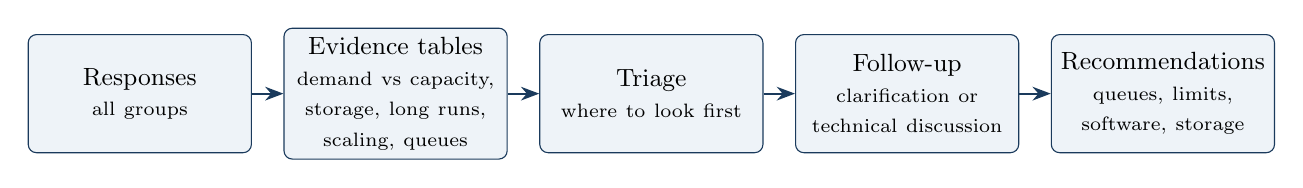
\begin{tikzpicture}[node distance=0.4cm,
      box/.style={draw=iiser,fill=soft,rounded corners=3pt,align=center,font=\small,text width=2.6cm,minimum height=1.5cm},
      arr/.style={-{Stealth},thick,iiser}]
    \node[box] (r) {Responses\\{\scriptsize all groups}};
    \node[box,right=of r] (e) {Evidence tables\\{\scriptsize demand vs capacity, storage, long runs, scaling, queues}};
    \node[box,right=of e] (t) {Triage\\{\scriptsize where to look first}};
    \node[box,right=of t] (f) {Follow-up\\{\scriptsize clarification or technical discussion}};
    \node[box,right=of f] (p) {Recommendations\\{\scriptsize queues, limits, software, storage}};
    \foreach \a/\b in {r/e,e/t,t/f,f/p} \draw[arr] (\a) -- (\b);
  \end{tikzpicture}}
  \vfill
  \small
  \begin{tabularx}{\textwidth}{@{}l X@{}}
    \multicolumn{2}{@{}l}{\textbf{Triage suggestions}} \\
    1 --- characterised & the information is sufficient; nothing further needed \\
    2 --- clarification & a short follow-up resolves a gap or an inconsistency \\
    3 --- technical look & an unusual requirement is discussed with the group, with proportionate evidence \\
  \end{tabularx}
\end{frame}

\begin{frame}{Principles of the evaluation}
  \begin{itemize}
    \item No scores, no rankings, no automatic queue assignment.
    \item ``Don't know'' and missing data are never counted against a group.
    \item Answers that do not fit together become \textbf{questions to the group}, not findings.
    \item Comparisons with other sources (e.g.\ scheduler records, code documentation) are made by people, openly.
    \item Unusual requirements call for evidence in proportion --- just as ordinary ones are characterised by evidence.
  \end{itemize}
\end{frame}

\begin{frame}{Timeline and contacts}
  \begin{itemize}
    \item The form will be shared in a few days
    \item Department contacts will be informed when it opens
  \end{itemize}
  \vfill
  \centering
  \textcolor{iiser}{Thank you for helping us understand the range of computing work at IISER Bhopal,\\
  so that services can be designed to serve it fairly.}
\end{frame}

\end{document}
